% Copyright (C) 2010,2011,2012,2013,2014,2015,2016 The ESPResSo project
% Copyright (C) 2002,2003,2004,2005,2006,2007,2008,2009,2010 
%   Max-Planck-Institute for Polymer Research, Theory Group
%  
% This file is part of ESPResSo.
%   
% ESPResSo is free software: you can redistribute it and/or modify it
% under the terms of the GNU General Public License as published by the
% Free Software Foundation, either version 3 of the License, or (at your
% option) any later version.
%  
% ESPResSo is distributed in the hope that it will be useful, but
% WITHOUT ANY WARRANTY; without even the implied warranty of
% MERCHANTABILITY or FITNESS FOR A PARTICULAR PURPOSE.  See the GNU
% General Public License for more details.
%  
% You should have received a copy of the GNU General Public License
% along with this program.  If not, see <http://www.gnu.org/licenses/>.
%
\documentclass[
a4paper,                        % paper size
11pt,                           % font size
twoside,                        % two sided
footsepline,                    % add a line to separate the footer
headsepline,                    % add a line to separate the header
headexclude,                    % header does not belong to the text
footexclude,                    % footer does not belong to the text
pagesize,                       % set the pagesize in a DVI document
]{scrartcl}

% Copyright (C) 2010,2011,2012 The ESPResSo project
% Copyright (C) 2002,2003,2004,2005,2006,2007,2008,2009,2010
%  Max-Planck-Institute for Polymer Research, Theory Group
%  
% This file is part of ESPResSo.
%   
% ESPResSo is free software: you can redistribute it and/or modify it
% under the terms of the GNU General Public License as published by the
% Free Software Foundation, either version 3 of the License, or (at your
% option) any later version.
%  
% ESPResSo is distributed in the hope that it will be useful, but
% WITHOUT ANY WARRANTY; without even the implied warranty of
% MERCHANTABILITY or FITNESS FOR A PARTICULAR PURPOSE.  See the GNU
% General Public License for more details.
%  
% You should have received a copy of the GNU General Public License
% along with this program.  If not, see <http://www.gnu.org/licenses/>.
%
\usepackage[draft]{varioref}    % defines \vref
\usepackage{hyperref}           % automatically creates links when
                                % using pdflatex, defines \url
\usepackage{ifpdf}              % defines \ifpdf
\usepackage{graphicx}           % handles graphics
\usepackage{color}              % use colors

\usepackage{amsmath}

\usepackage{verbatim}           % required for \verbatim and \endverbatim
\usepackage{fancyvrb}
\usepackage{calc}               % compute length
\usepackage{ifthen}             % provide ifthen
\usepackage{xspace}
\usepackage{units}
\usepackage[numbers]{natbib}

% For building the distribution docs, disable todo boxes.
%\usepackage[disable]{todonotes}
\usepackage{todonotes}

\newcommand{\es}{\mbox{\textsf{ESPResSo}}\xspace}
\newcommand{\ie}{\textit{i.e.}\xspace}
\newcommand{\eg}{\textit{e.g.}\xspace}
\newcommand{\etal}{\textit{et al.}\xspace}

\newcommand{\codebox}[1]%
{\texttt{#1}}

\DefineVerbatimEnvironment{code}{Verbatim}%
{commandchars=\\\{\}}
\makeatletter
\newenvironment{tclcode}
{%
  \addtolength{\linewidth}{-2em}% set the line length
  \@minipagetrue%%%DPC%%%
  \@tempswatrue%%%DPC%%%
  \hsize=\linewidth%
  \setbox0=\vbox\bgroup\verbatim
}{\endverbatim
  \unskip\setbox0=\lastbox%%%DPC%%%
  \egroup
  \par%
  \noindent\hspace{1em}%
  \codebox{\box0}%
  \par\noindent%
}
\makeatother

% \newcommand{\todo}[1]{
%   \marginpar{%
%     \setlength{\fboxrule}{1pt}
%     \fcolorbox{red}{yellow}{%
%       \parbox{\marginparwidth-2\fboxrule-2\fboxsep}{%
%         \bf\raggedright\scriptsize #1%
%       }%
%     }%
%   }%
% }

\makeatletter
\renewcommand{\minisec}[1]{\@afterindentfalse \vskip 1.5ex
  {\parindent \z@
    \raggedsection\normalfont\sffamily\itshape\nobreak#1\par\nobreak}%
  \@afterheading}
\makeatother

\newcommand{\esptitlehead}{
  \titlehead{
    \begin{center}
      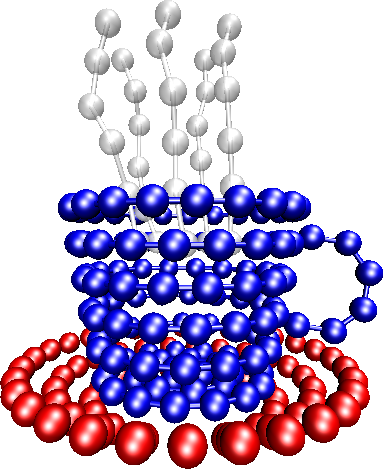
\includegraphics[width=5cm]{logo/transparentbg}
    \end{center}
  }
}


\lstset{language=Python} 

\begin{document}
\esptitlehead
\title{Tutorial 2: A simple charged system%
\ifdefined\esversion%
\thanks{For \es \esversion}%
\fi%
}

\maketitle
\tableofcontents

\section{Introduction}

This tutorial introduces some of the features of \es\ by constructing
step by step a simulation script for a simple salt crystal.  We cannot
give a full Python tutorial here; however, most of the constructs should
be self--explanatory. We also assume that the reader is familiar with
the basic concepts of a MD simulation here. The code pieces can be
copied step by step into a file, which then can be run using
\verb|pypresso <file>| from the \es source directory.

\section{Basic set up}

Our script starts with setting up the initial configuration.  Most
conveniently, one would like to specify the density and the number of
particles of the system as parameters:

\begin{tclcode}
# Set system parameters
n_part = 200
density = 0.7
box_l = (n_part/density)**(1./3.)
\end{tclcode}

These variables do not change anything in the simulation engine, but
are just standard Python variables; they are used to increase the
readability and flexibility of the script. The box length is not a
parameter of this simulation; it is calculated from the number of
particles and the system density. This allows to change the parameters
later easily, e.~g.\ to simulate a bigger system.

The parameters of the simulation engine are modified by changing the
espressomd.System() properties.

\begin{tclcode}
# Setup system geometry in Espresso
system = espressomd.System()

system.box_l = [box_l, box_l, box_l]
system.periodicity = [1, 1, 1]
\end{tclcode}

These lines define for example a cubic simulation box of size 
\verb|box_l|, and periodic boundary conditions in all spatial dimensions. 
We now fill this simulation box with particles

\begin{tclcode}
# Place particles
q = 1.
ptype = 0

for i in xrange(n_part):
    q *= -1
    ptype = 1-ptype
    system.part.add(id=i, type=ptype, 
                    pos=numpy.random.random(3) * system.box_l, q=q)
\end{tclcode}

This loop adds \verb|n_part| particles at random positions, one by
one.  In this construct, the \verb|part| command is used to specify 
particle properties, here the position, the charge \verb|q| and the type. 
In \es\ the particle type is just an integer number which allows to group
particles; it does not imply any physical parameters. Here we 
alternate between creating positive charges of type 0 and negative
charges of type 1.

Now we define the ensemble that we will be simulating. This is done
using the \verb|thermostat| class. We also set some integration
scheme parameters:

\begin{tclcode}
# Simulation parameters
system.time_step = 0.01
system.cell_system.skin = 0.3

# Thermostat
temp = 1.
gamma = 1.
thermostat.Thermostat().set_langevin(kT=temp, gamma=gamma)
\end{tclcode}

This switches on the Langevin thermostat for the NVT ensemble, with
temperature \verb|temp| and friction coefficient \verb|gamma|. The skin depth
\verb|skin| is a parameter for the link--cell system which tunes its
performance, but shall not be discussed here.

Before we can really start the simulation, we have to specify the
interactions between our particles.  We use a simple, purely repulsive
Lennard-Jones interaction to model a hard core repulsion. Additionally the
charges interact via the Coulomb potential:

\begin{tclcode}
# Lennard-Jones interactions
lj_sig = 1.
lj_eps = 1.
lj_cut = 2.**(1. / 6.)
system.non_bonded_inter[0, 0].lennard_jones.set_params(
    epsilon=lj_eps, sigma=lj_sig, cutoff=lj_cut, shift="auto")
system.non_bonded_inter[1, 0].lennard_jones.set_params(
    epsilon=lj_eps, sigma=lj_sig, cutoff=lj_cut, shift="auto")
system.non_bonded_inter[1, 1].lennard_jones.set_params(
    epsilon=lj_eps, sigma=lj_sig, cutoff=lj_cut, shift="auto")

p3m = electrostatics.P3M(bjerrum_length=10.0, accuracy=1e-3)
system.actors.add(p3m)
\end{tclcode}

The first three \verb|non_bonded_inter| commands instruct \es\ to use the same
purely repulsive Lennard--Jones potential for the interaction between
all combinations of the two particle types 0 and 1; by using different
parameters for different combinations, one could simulate differently
sized particles.  The last two lines set the Bjerrum length to the value
10, and then instructs \es\ to use the P$^3$M method for the Coulombic
interaction and to try to find suitable parameters for an rms force
error below $10^{-3}$, with an optimal mesh size. This command will also print 
the parameters and timings that the tuning found to the screen. Tuning takes 
some time; if you run many simulations with similar parameters, you might want 
to save and reload
the P$^3$M parameters. You can obtain the P$^3$M parameters by
\verb|get_params()|:

\begin{tclcode}
p3m_params = p3m.get_params()
for key in p3m_params.keys():
    print("{} = {}".format(key, p3m_params[key]))
\end{tclcode}


\section{Running the simulation}

Now we can integrate the particle trajectories for a couple of time
steps:

\begin{tclcode}
integ_steps = 200
int_n_times = 20

# Main integration loop
for i in xrange(int_n_times):
    temp = system.analysis.energy()['ideal'] / ((3 / 2.0) * n_part)
    print("t={0}, E={1}, T={2}".format(system.time,
                                       system.analysis.energy()['total'], temp))
    system.integrator.run(integ_steps)
\end{tclcode}

This code block is the primary simulation loop and runs
$20\times$\verb|integ_steps| MD steps. Every \verb|integ_steps| time
steps, the potential, electrostatic and kinetic energies are printed
out. The latter one is printed as temperature, by rescaling by the
number of degrees of freedom (3) multiplied by $1/2kT$. Note that
energies are measured in $kT$, so that only the factor $1/2$
remains. Also note that $3/2$ should be written as $3/2.0$; to ensure
that Python does not perform integer division (resuting in $1$ instead of
$1.5$).

Note, that in \es\ there are usually 3 translational degrees per
particle. However, if \verb|ROTATION| is compiled in, there are in
addition 3 rotational degrees of freedom, which also contribute to the
kinetic energy.  You can get this number in the following way:

\begin{tclcode}
if "ROTATION" in code_info.features():
    deg_free = 6
else:
    deg_free = 3
\end{tclcode}

Then all you need to do is to replace the hardcoded 3 by \verb|deg_free|.

However, if you run the simulation, it will still
crash: \es\ complains about particle coordinates being out of range.
The reason for this is simple: Due to the initial random setup, the
overlap energy is around a million $kT$, which we first have to remove
from the system. In \es, this can be accelerated by limiting the maximum
forces, i.~e.\ modifying the Lennard--Jones force such that it is
constant below a certain distance. Before the main integration loop, we
therefore insert this equilibration loop:

\begin{tclcode}
integ_steps = 200

# Warmup integration loop
for cap in xrange(20, 200, 20):
    print("t={0}, E={1}".format(system.time,
                                system.analysis.energy()['total']))
    system.non_bonded_inter.set_force_cap(cap)
    system.integrator.run(integ_steps)
system.non_bonded_inter.set_force_cap(0)
\end{tclcode}

This loop integrates the system with a force cap value of initially 20 and
finally 180.  The last command switches the force cap off again. With
this equilibration, the simulation script runs fine. As a check
that the equilibration loop works correctly, you might want to copy the
energy and force printing from the main integration loop. You can then
observe how the temperature initially overshoots and is then relaxed to
its target value by the thermostat.

\section{Writing out data}

For later analysis of the simulation results, one will
usually like to write out simulation data to configuration files.
For this purpose one can use the \verb|cPickle| Python library to 
write simulation data to a file in an easily parseable form.  We add the 
following lines to the integration loop just after the \verb|integrator.run| line
in order to write out the system configuration files
``config\_0'' through ``config\_19'':

\begin{tclcode}
    # Pickle particle data
    with open("config_{}".format(i), "w") as configfile:
        pickle.dump(system.part, configfile, -1)
\end{tclcode}

In order to write out \verb|System()| variables such as the boxlength 
\verb|box_l|, the timestep \verb|time_step| or the skin \verb|skin| to the 
file ``system\_config'', one can insert the following lines before or after the 
main loop integration:

\begin{tclcode}
# Pickle system properties
with open("system_config", "w") as system_config:
    pickle.dump(system, system_config, -1)
\end{tclcode}


Reading the system variables is done by the following simple script:

\begin{tclcode}
# Import system properties
system = espressomd.System()
pickle.load(open("system_config","r"))
\end{tclcode}

The \verb|load()| command will set the system variables
to the values specified in the file. This includes to set for example 
the box dimensions for the simulation. Note that it is important to have the box 
dimensions set before reading the particles, to avoid problems with the periodic 
boundary conditions. The particles (including all properties) of the first 
frame can be restored with the following line:

\begin{tclcode}
# Import of particle properties
pickle.load(open("config_0","r"))
\end{tclcode}


\begin{figure}[tb]
  \centering
  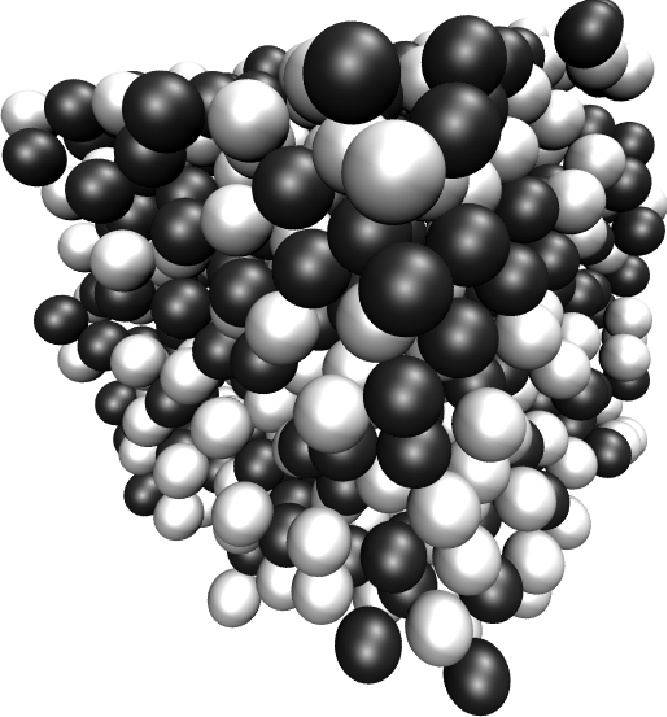
\includegraphics[width=0.4\textwidth]{figures/salt}
  \caption{VMD Snapshot of the salt system}
  \label{fig:snapshot}
\end{figure}

The \verb|pickle| mechanism is typically used for one of two main
purposes, checkpointing and offline analysis.
Checkpointing is useful for long-running simulations: If you have
a simulation that runs for several days, you may want to have it
periodically write its current state to a file. That way, the
simulation can be resumed if your computer crashes while the
simulation is running.
Offline analysis refers to analyzing physical parameters of the
simulation after the simulation has finished and will be discussed in
the next section.

\section{Analysis}

Having written out pickle files during the simulation, we can now
investigate the system. As an example, we will create a second script which 
calculates the averaged radial distribution functions $g_{++}(r)$ and 
$g_{+-}(r)$. The radial distribution function for the current 
configuration can be calculated using the \verb|rdf()| command from the 
\verb|analysis| submodule:

\begin{tclcode}
    # Calculate rdf
    rdf_bins = 100
    rdf_list_a = [0]
    rdf_list_b = [1]
    r, rdf = system.analysis.rdf(rdf_type='rdf', type_list_a=rdf_list_a,
                                 type_list_b=rdf_list_b, r_min=0.9,
                                 r_max=system.box_l[0] / 2., r_bins=rdf_bins)
\end{tclcode}


The shown \verb|rdf()| command returns the distribution function
of particles of type 1 around particles of type 0 (i.~e.\ of opposite
charges) for radii between $0.9$ and half the box length, subdivided
into $100$ bins.  Changing \verb|rdf_list_a| and \verb|rdf_list_b| to either 
[0] and [0] or [1] and [1] allows to determine the distribution of equal charges
around each other. The result are two numpy arrays containing the of $r$ and 
$g(r)$ values.
After the system properties are loaded, we loop additionally over all pickle 
files given as command line arguments to average over all configurations.

\begin{tclcode}
# Import system properties
system = espressomd.System()
pickle.load(open("system_config", "r"))

rdf_bins = 100
rdf_list_a = [0]
rdf_list_b = [1]

# Initialize the total RDF with zero
cnt = 0
avg_rdf = numpy.zeros(rdf_bins)

for filename in sys.argv[1:]:
    # Import of particle properties
    try:
        pfile = open(filename, "r")
        pickle.load(pfile)
        pfile.close()
    except Exception as e:
        print("Could not import particles from '{}'.".format(filename))
        print(e)
        continue

    # Calculate rdf
    r, rdf = system.analysis.rdf(rdf_type='rdf', type_list_a=rdf_list_a,
                                 type_list_b=rdf_list_b, r_min=0.9,
                                 r_max=system.box_l[0] / 2., r_bins=rdf_bins)
    avg_rdf += rdf

    system.part[:].remove()

    cnt += 1

avg_rdf *= 1. / cnt
\end{tclcode}

Initially, the sum of all $g(r)$, which is stored in \verb|avg_rdf|,
is set to 0.  Then the loops over all configurations given by
\verb|sys.argv|, calculates $g(r)$ for each configuration and adds up all
the $g(r)$ in \verb|avg_rdf|.  Finally, this sum is normalized by
dividing by the number of configurations. Note again the
\verb|1. / cnt|; also here, this is necessary, since \verb|1 / cnt| is 
interpreted as an integer division, which would result in 0 for $\text{cnt}>1$. 
 \verb|sys.argv| is a predefined variable: it contains all the command line 
parameters. Therefore this script should be called like this:
\begin{verbatim}
  ./pypresso <script> config_*
\end{verbatim}

\begin{figure}[tb]
  \centering
  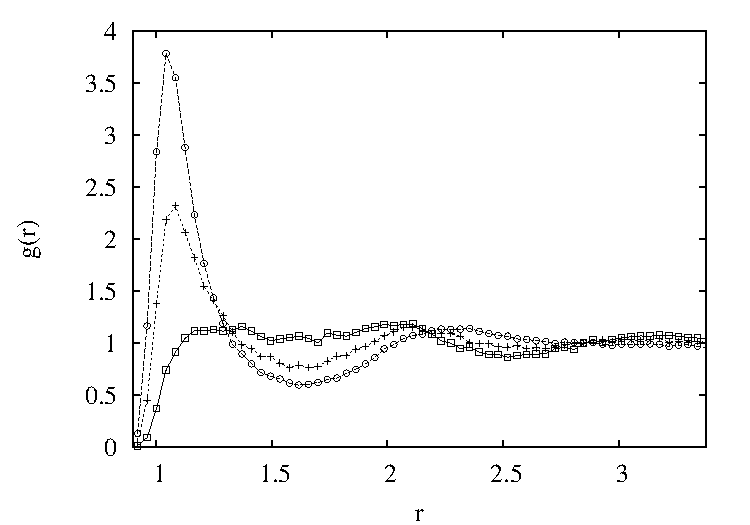
\includegraphics[width=0.7\textwidth]{figures/nacl-rdf}
  \caption{Radial distribution functions $g_{++}(r)$ between equal
    charges (rectangles) and $g_{+-}(r)$ for opposite charges
    (circles). The plus symbols denote $g(r)$ for an uncharged
    system.}
  \label{fig:rdf}
\end{figure}

The printing of the calculated radial distribution functions is
simple. Add to the end of the previous snippet the following lines:

\begin{tclcode}
# Write averaged data to plot file
plot = open("rdf.data", "w")
plot.write("# r\trdf(r)\n")
for i in xrange(len(rdf)):
    plot.write("{0}\t{1}\n".format(r[i], avg_rdf[i]))
plot.close()
\end{tclcode}

This instructs Python to write the \verb|avg_rdf| to the
file \verb|rdf.data| in gnuplot--compatible format. Fig.~\ref{fig:rdf}
shows the resulting radial distribution functions, averaged over 100
configurations. In addition, the distribution for a neutral system is
given, which can be obtained from our simulation script by simply
removing the commands

\begin{tclcode}
    p3m = electrostatics.P3M(bjerrum_length=10.0, accuracy=1e-3)
    system.actors.add(p3m)
\end{tclcode}

and therefore not turning on P$^3$M.
To plot your own results, run \verb|gnuplot| in a Terminal window
and type the following:
\begin{tclcode}
plot "rdf.data" using 1:2	
\end{tclcode}
If you have written out RDFs for multiple combinations of species,
you can plot them into one graph like this:
\begin{tclcode}
plot "rdf00.data" using 1:2 w l title "g++", \
     "rdf11.data" using 1:2 w l title "g--", \
     "rdf01.data" using 1:2 w l title "g+-"	
\end{tclcode}


\section{Further ideas}

The code example given before is still quite simple, and the reader is
encouraged to try to extend the example a little bit, e.~g. by using
differently sized particle, or changing the interactions. If something
does not work, \es\ will give comprehensive error messages, which
should make it easy to identify mistakes. For real simulations, the
simulation scripts can extend over thousands of lines of code and
contain automated adaption of parameters or online analysis, up to
automatic generation of data plots.  Parameters can be changed
arbitrarily during the simulation process, as needed for e.~g.\
simulated annealing. The possibility to perform non--standard
simulations without the need of modifications to the simulation core
was one of the main reasons why we decided to use a script language
for controlling the simulation core.

%\section{Accelerating the simulation using a GPU}

%TODO
\iffalse
\es{} can make use of an Nvidia graphics processing unit (GPU) for 
accelerating simulations.
Of course, we expect that results of the GPU-based implementation of
P$^3$M to be exactly identical to those of the traditional CPU
implementation. So copy the results from the previous task to a
different file name (e.g.~\verb|rdf_p3m_cpu.data|) for comparison.
Additionally, we'd like to find out exactly how much faster the GPU
implementation is. So first wrap your previous simulation script with
a time measurement, run it again and note down the execution time.
\begin{tclcode}
	set starttime [clock seconds]
	
	# previous script code goes here
	
	set endtime [clock seconds]
	puts "Simulation took [expr $endtime-$starttime] seconds"	
\end{tclcode}

To switch to the GPU-based implementation of 
P$^3$M, go to the line of your simulation script that contains
\verb|inter coulomb| and replace \verb|p3m| with \verb|p3m gpu|.
Then run the simulation again and note down the execution time,
which should be a lot shorter now. Plot the RDFs from both
the CPU and the GPU simulation into one graph and check whether the
results agree.
\fi

%\section{Using the MEMD algorithm}

%TODO
\iffalse
\es{} provides a variety of different electrostatics solvers. So far,
we have been introduced to P$^3$M, but in this section we will try
something new. A fairly recent addition to the family of electrostatics
solvers is the "Maxwell Equations Molecular Dynamics" (MEMD) algorithm.
To use it, two parameters have to be set: A mesh size, and a method
parameter called \verb|f_mass|, which can be estimated by a formula
given in the \es{} user guide. In this example, a good estimate for
the mesh size is 12, but this can be varied, affecting speed and
accuracy of the algorithm.

The MEMD algorithm relies on a very specific spatial distribution of
the particles across processors, and will therefore currently not work
with Verlet lists. Since those are switched on by default, they will
have to be turned off manually by adding the following line before the
\verb|setmd| commands:

\begin{tclcode}
  cellsystem domain_decomposition -no_verlet_list
\end{tclcode}


Besides this, you will have to replace the initialization of the
P$^3$M interaction (\verb|inter| \verb|coulomb|...) with an
appropriate one for MEMD:

\begin{tclcode}
  set memd_mesh 12
  set f_mass [expr 100.0*pow( ([setmd time_step]*$memd_mesh/$box_l),2.0)]
  inter coulomb 10.0 memd $f_mass $memd_mesh
\end{tclcode}


In the example script included
within the \es{} code, there is already an \verb|if|-construct 
provided and you can switch between the methods at the very top
of the script.

You can copy the results from your completed tasks so far to a different
filename (e.g.~\verb|rdf_p3m.data|) for comparison. Then, just
run the simulation and analysis again, and compare the speed and 
resulting radial distribution function of the two methods.
\fi

%\section{Partially periodic boundary conditions}

%TODO
\iffalse
\begin{figure}[h]
  \centering
  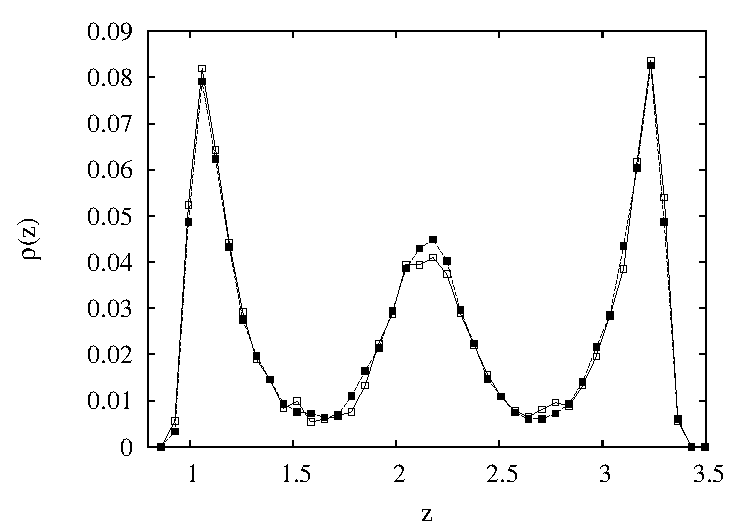
\includegraphics[width=0.7\textwidth]{figures/neutral-rho}
  \caption{Distribution of positive charges $\rho_+(z)$ (open squares)
    and of negative charges $\rho_-(z)$ (closed squares) under
    confinement along $z$.}
  \label{fig:neutralrho}
\end{figure}

One of the strengths of \es{} is the possibility to simulate charged
systems with partially periodic boundary conditions.
Before you proceed, check your \emph{myconfig.hpp} file to make
sure that the \verb|PARTIAL_PERIODIC| feature is enabled.

As an example of a system in partially-periodic boundary conditions,
we will modify our script to simulate our simple salt in a slit pore.
Remove the \verb|cellsystem|, \verb|setmd box_l| and \verb|setmd periodic| lines left
over from your previous simulation simulation script and replace them
with these lines:

\begin{tclcode}
  set box_lxy [expr sqrt(2)*$box_l]
  set box_lz  [expr 0.5*$box_l]
  setmd box_l $box_lxy $box_lxy [expr $box_lz + 1.0]
  setmd periodic 1 1 0
  constraint wall normal 0 0  1 dist 0 type 2
  constraint wall normal 0 0 -1 dist [expr -$box_lz - 1.0] type 2
\end{tclcode}

The final two lines add two confining walls at the top
and the bottom of the simulation box. The wall is given by its normal
vector (pointing up and downwards here), and its distance from
$(0,0,0)$. Therefore this defines one wall at $z=0$, and a second
one at $z=$\verb|box_lz|$+1$. Finally, the type of the wall is used like a
particle type to define the interaction of the walls with the particles.

The addition of $1.0$ to the slit width is due to the fact that we will
use a Lennard-Jones potential to model the wall; this means that
particles of diameter $1.0$ cannot come closer than $1.0$ to the wall. In a
way, the wall itself therefore has a thickness of $0.5$. To compensate
for this, we simply make the box bigger by 1.

We also need to choose the initial positions of our particles to match
the new box dimensions. Replace the appropriate part of your
simulation script with this random drawing of particle positions:

\begin{tclcode}
  set posx [expr $box_lxy*[t_random]]
  set posy [expr $box_lxy*[t_random]]
  set posz [expr ($box_lz-1.0)*[t_random] + 1.0]
\end{tclcode}

When defining the interactions, we now also need to add the
interactions between the particles and the walls, which is the same as
between the particles:

\begin{tclcode}
  inter 0 2 lennard-jones $eps $sig $cut $shift 0
  inter 1 2 lennard-jones $eps $sig $cut $shift 0
\end{tclcode}

For the electrostatic part, we also need to choose a different algorithm,
as P$^3$M can only handle fully periodic boundary conditions. We
choose the MMM2D method:

\begin{tclcode}
  cellsystem layered 3
  inter coulomb 1.0 mmm2d 1e-4  
\end{tclcode}

which replaces the \verb|inter coulomb 10.0 p3m ...| code. Note the
decreased Bjerrum length --- the confined system would take too long for
a tutorial to equilibrate with Bjerrum length 10.0. Still,
equilibrating the system is now more difficult. First, we cannot
simply ramp up all Lennard-Jones interactions anymore; otherwise,
particles will penetrate the walls and break the confinement. Second,
we need to ramp up the electrostatic interaction more carefully
now. The following code replaces the equilibration loop previously 
used. It gradually increases the Bjerrum length to the
target value of 1.0, and caps only the Lennard-Jones interactions
between the particles. The latter can be done by switching on
individual force capping, and setting a force cap radius for the
particle-particle interactions:

\begin{tclcode}
inter forcecap individual
for {set i 1} {$i < 10} {incr i} {
    set rad [expr 1.0 - 0.5*$i/10.0]
    set lb [expr 1.0 * $i / 10.0]
    inter 0 0 lennard-jones $eps $sig $cut $shift 0 $rad
    inter 1 0 lennard-jones $eps $sig $cut $shift 0 $rad
    inter 1 1 lennard-jones $eps $sig $cut $shift 0 $rad
    inter coulomb $lb mmm2d 1e-4
    integrate $integ_steps
}
inter forcecap 0
inter coulomb 1.0 mmm2d 1e-4  
\end{tclcode}

Finally, when writing out, we should update the set of
Tcl-variables to represent the asymmetric box, and write out
\verb|box_lxy| and \verb|box_lz| instead of just \verb|box_l|.

\subsection*{Analysis}

For a such a strongly confined system, the radially averaged
distribution function is inappropriate. Instead, it would be more
interesting to study the distribution of the particles along the slit
width. \es{}  does not provide such a function, however, we can easily
write one using the \verb|bin| command, which simply allows us 
to create a histogram based on a set of values given as a Tcl list.
Therefore, we first create the list
of z-coordinates, and then bin them:

\begin{tclcode}
  set bins 20
  set data ""
  for {set p 0} {$p <= [setmd max_part]} {incr p} {
    lappend data [lindex [part $p pr pos] 2]
  }
  set rho [bin -linbins 0.5 [expr $box_lz + 0.5] $bins $data]
\end{tclcode}

Here, \verb|bins| is a variable that you should set to the desired
number of bins (20 should be fine). Otherwise, this code can replace
the analyze rdf command. The \verb|bin| command can also be used to
calculate the coordinates of the bins:

\begin{tclcode}
  bin -linbins 0.5 [expr $box_lz + 0.5] $bins -binctrwdth
\end{tclcode}

will return a list of the centers and widths of the bins, which can be
used in analogy to \verb|rlist| in the previous analysis code. Of
course, it would be interesting to study the distribution of positive
and negative charges separately; for this, you need to duplicate the
averaging code, and use two data sets to append the z-coordinates to,
depending on the particle type:

\begin{tclcode}
  if {[part $p pr type] == 0} {
    lappend data0 [lindex [part $p pr pos] 2]
  } {
    lappend data1 [lindex [part $p pr pos] 2]
  }
\end{tclcode}

The resulting distribution of charges is shown in
Fig.~\ref{fig:neutralrho}. You can see a layering effect of the
confinement on the charge distributions.

\begin{figure}[h]
  \centering
  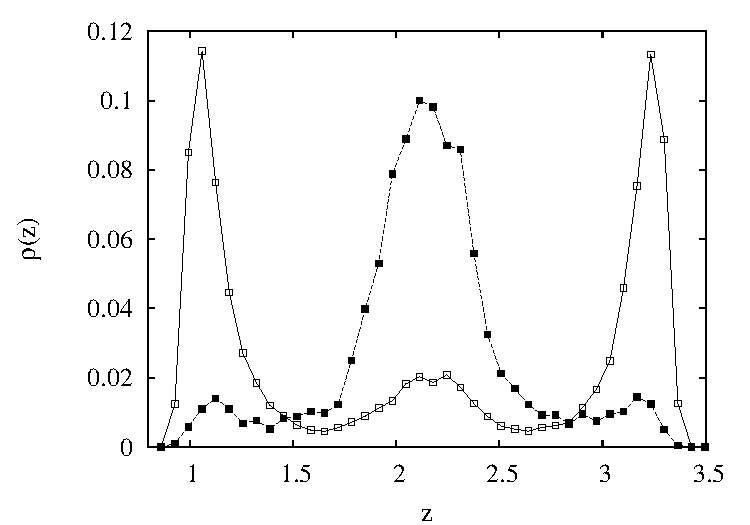
\includegraphics[width=0.7\textwidth]{figures/nonneutral-rho}
  \caption{Distribution of positive charges $\rho_+(z)$ (open squares)
    and of negative charges $\rho_-(z)$ (open squares) under
    confinement along $z$. The two confining walls are negatively
    charged, pushing away the negative charges.}
  \label{fig:nonneutralrho}
\end{figure}

\subsection*{Charging the walls}

So far, the distributions of particles of type 0 and 1 are more or
less the same, as one would expect. However, we can change this by
introducing charged walls. That is done using the
\verb|constraint plate| command:

\begin{tclcode}
  set sigma [expr -0.25*$n_part/($box_lxy*$box_lxy)]
  constraint plate height 0 sigma $sigma
  constraint plate height [expr $box_lz + 1.0] sigma $sigma
\end{tclcode}

Note that you need to have both the \verb|constraint plate| and the 
\verb|constraint wall| commands in your simulation script.
This adds two plates at the bottom and top of the simulation box. The
charged walls (the capacitor \emph{plates}) are necessarily
perpendicular to the z-axis, since for all electrostatics methods for
2d-periodic systems, \es{} assumes that the z-axis is the
non-periodic axis.

Note that
this adds two walls with a total charge of \verb|n_part|/2, which
would make the overall system charged. So to maintain charge
neutrality, we need to only create half of the charges (i.e. 100)
with alternating charges as before, while the rest is created
with positive charge.
For this system, you should obtain distributions as shown in
Fig.~\ref{fig:nonneutralrho}. The distribution of charges differs
strongly between the two types of charges; while the positive charges
layer at the walls, the negative charges accumulate in the center of
the system.
\fi

\end{document}
